%
% oblique.tex -- normal derivative for oblique boundary
%
% (c) 2019 Prof Dr Andreas Müller, Hochschule Rapperswil
%
\documentclass[tikz,12pt]{standalone}
\usepackage{amsmath}
\usepackage{times}
\usepackage{txfonts}
\usepackage{pgfplots}
\usepackage{csvsimple}
\usetikzlibrary{arrows,intersections,math}
\begin{document}
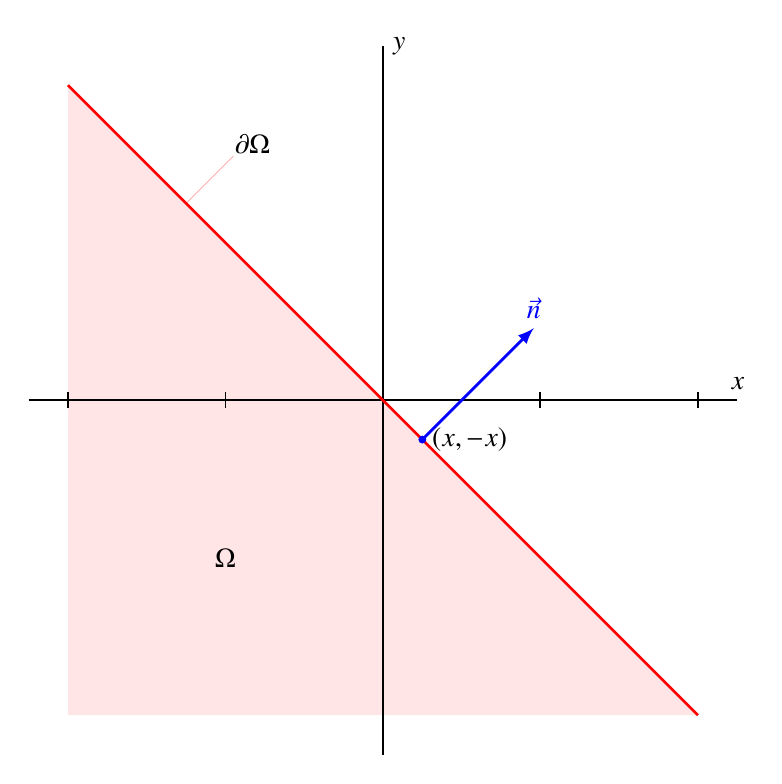
\begin{tikzpicture}[>=latex]

\fill[color=red!10] (-4,-4)--(4,-4)--(-4,4)--cycle;

\draw[line width=0.7pt] (-4.5,0)--(4.5,0) coordinate[label={$x$}];
\draw[line width=0.7pt] (0,-4.5)--(0,4.5) coordinate[label={right:$y$}];

\draw[line width=0.7pt] (-4,-0.1)--(-4,0.1);
\draw[line width=0.7pt] (-2,-0.1)--(-2,0.1);
\draw[line width=0.7pt] (2,-0.1)--(2,0.1);
\draw[line width=0.7pt] (4,-0.1)--(4,0.1);

\draw[color=red,line width=1pt] (-4,4)--(4,-4);

\node at (-2,-2) {$\Omega$};
\node at (-2,3) [above right] {$\partial\Omega$};
\draw[line width=0.1pt,color=red] (-2.5,2.5)--(-1.9,3.1);

\fill[color=blue] (0.5,-0.5) circle[radius=0.05];
\draw[->,color=blue,line width=1pt] (0.5,-0.5)--({0.5+sqrt(2)},{-0.5+sqrt(2)});
\node[color=blue] at ({0.5+sqrt(2)},{-0.5+sqrt(2)}) [above] {$\vec{n}$};
\node at (0.5,-0.5) [right] {$(x,-x)$};

\end{tikzpicture}
\end{document}

